\subsection{Spectrometer Array}
\label{Chap:Methods:subsec:GammaSpec}

\subsubsection{Experimental Setup}
A long array of scintillating crystals is placed in the beam path and its scintillation light is measured with a CCD. The spectrum of gamma radiation passing through the crystals can be inferred by simulating the response of the array in GEANT4 \cite{GEANT4} and comparing it to the response measured in the experiment \cite{Behm2018_Gamma}.
A conceptual sketch of the experimental setup is shown in Figure \ref{Methods:Figs:SketchGammaSpec}: a beam of gamma rays (green) enters from the left side of the sketch, passes through a vacuum window (orange) into air, then traverses a lead collimator and enters the scintillator array. The crystals are indicated in yellow. The response of the detector is imaged by a camera (bottom right corner). 

\begin{figure}
\centering
\includegraphics[width=0.8\columnwidth]{GammaSpectrometerSketch.pdf}
\caption[Sketch of a gamma spectrometer setup in an experiment.]{Sketch of a gamma spectrometer setup in an experiment. The gamma rays (green) traverse from the left a vacuum window (orange) and then in air through a lead collimator onto an array of scintillators (yellow) housed in a casing. The stack is predominantly extended in the longitudinal direction (z) but can also resolve one transverse dimension (here y). A camera directly images the open side of the scintillator array.}
\label{Methods:Figs:SketchGammaSpec}
\end{figure}

The individual scintillators are caesium-iodide crystals doped with thallium, with the spatial dimensions $5 \times 5 \times 50\,\mathrm{mm}$. 
The long side of the crystals is oriented transversely to the propagation direction of the gamma rays ($z$), in the sketch shown in Figure \ref{Methods:Figs:SketchGammaSpec} this is the horizontal axis $x$ (see also Figure \ref{Methods:Figs:GammaSpectrometer_Axes}). This maximises the light yield as the response of the detector is integrated along this axis ($x$) but at cost of spatial resolution. The crystals are arranged in a two-dimensional grid of columns ($z$) and rows ($y$). Crystals along the longitudinal axis $z$ measure the decay of the radiation and can be used to infer the spectrum. The response in the $y$-axis encodes the vertical divergence of the radiation. 

The crystals are separated from each other by light-tight spacers such that each crystal is enclosed from all but one side, from which the scintillation light leaves the crystal. This crystal side faces in $x$ direction and the scintillation light is measured on a CCD. In all the experiments discussed in this thesis cooled 14-bit EMCCD cameras of type Andor iXon were used, which are very sensitive and allow for high gain but in turn also require efficient light shielding. The cameras were equipped with suitable objectives and bandpass filters that only transmit light in the bandwidth of the scintillation light at a wavelength of $546\pm10\nm$. A reflective casing for the crystals along with polishing and reflective coating of the crystals can increase the light output. The material and thickness of the dividers between the crystal columns determine how fast the incoming radiation decays which can be used to `tune' the response of the detector to the right spectral range. The separation and thickness of the crystals in the $y$-axis, on the other hand, determines the vertical spatial or, with respect to the radiation source, the angular resolution.
\vspace{\baselineskip}

Two different scintillator stack designs were used as gamma spectrometers in the experiments described in this thesis. An overview of the dimensions and the materials used in the arrays is provided in Table \ref{Methods:GSpec:Table} and photos of the stacks are shown in Figure \ref{Methods:Figs:CsI_Stacks}. Examples of raw images from both detectors are shown in Figure \ref{Methods:Figs:CsI_shotexemp}.



\begin{figure}
\centering
\includegraphics[height=0.3\columnwidth]{scintillator.jpg}\hspace{2em}%
\includegraphics[height=0.3\columnwidth]{DualAxis_assembly.JPG}
\caption[Photographs of scintillator arrays used in experiments.]{Photographs of scintillator arrays used in experiments. Left: `RAL' stack of $47 \times 33$ crystals. Right: Long dual-axis stack consisting of $10 \times 70$ crystals. More details can be found in Table \ref{Methods:GSpec:Table}}
\label{Methods:Figs:CsI_Stacks}
\end{figure}

\begin{figure}
\centering
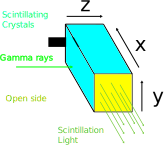
\includegraphics[height=0.3\columnwidth]{GammaSpecCrystals_2.pdf}\hspace{2em}%
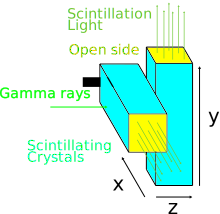
\includegraphics[height=0.3\columnwidth]{GammaSpecCrystals_3.pdf}
\caption[Sketch of crystal orientations in the spectrometer arrays relative to the incident gamma rays.]{Sketch of crystal orientations (cyan) in the spectrometer arrays relative to the incident gamma rays (green) for the RAL stack (left) and the alternating layers in the long dual-axis stack (right). The yellow faces indicate the open sides out of which the scintillation light (green) leaves the crystal.}
\label{Methods:Figs:GammaSpectrometer_Axes}
\end{figure}

In the experiment outlined in Chapter \ref{Chap:RR15} a $47 \times 33$ [longitudinal ($z$) $\times$ vertical ($y$)] array of crystals housed in an aluminium casing was used\footnote{Designed and built by Rob Clarke (CLF).} (see Figure \ref{Methods:Figs:CsI_Stacks}, left). The long side of the crystals was oriented along the horizontal direction ($x$) to maximise the light yield. The crystals were separated in $z$ and $y$ by 1-mm-thick light-tight aluminium spacers. On the sides ($x$) the array is held together by 1-mm-thick aluminium plates. One plate is solid, on the other side 4 mm diameter holes over the crystal faces allow the scintillation light to escape. The aluminium spacers and the solid plate reflect the light and direct the photons towards the only open side. The front and back side of the stack ($z$) are fortified with $9\,\mathrm{mm}$ thick steel plates.

The experiment described in Chapter \ref{Chap:BW} used the same scintillator array as above for the setup described in Chapter \ref{Chap:RR15}, but the thick steel front plate is replaced by a 1-mm sheet of plastic (PTFE) to reduce the attenuation of the incident radiation. In this setup a scintillating profile screen is placed in front of the spectrometer array (see previous section). The additional material of the profile screen roughly compensates the effect of the thinner front plate and matches the response of the detector to its previous configuration. 
\vspace{\baselineskip}


\begin{figure}
\centering
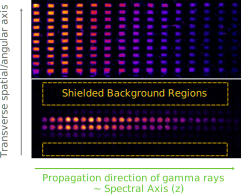
\includegraphics[width=.6\columnwidth]{GammaSpecExamples.pdf}
\caption[Examples of raw response recorded on scintillator arrays.]{Examples of raw response recorded on scintillator arrays in false colour, where black indicates low and orange a high signal. The radiation propagates into the stack from left to right, such that radiation of higher energy penetrate deeper into the stack. The vertical axis encodes spatial/angular information. Top: Top view of the first 15 crystal columns of the dual-axis stack. The response was measured at \textsc{Gemini} in 2019. Each square is an individual crystal, where the different dimensions are due to a large variation in the size of the transverse spacers that were used in the assembly. Top: Response of the `RAL' spectrometer stack to gamma radiation from inverse Compton scattering measured at \textsc{Gemini} in late 2015 (see Chapter \ref{Chap:RR15}). The stack was housed in a lead enclosure with a circular aperture (lead collimator) such that the signal area is restricted to the centre. The shielded regions can be used as background measurement. The crystals in this array have also rectangular faces but the casing holding the crystals in place has round apertures.}
\label{Methods:Figs:CsI_shotexemp}
\end{figure}


In the campaign described in Chapter \ref{Chap:linICS}, a longer array of $10 \times 70$ [transverse ($x,y$) $\times$ longitudinal ($z$)] crystals was fielded\footnote{Proposed by Stuart Mangles (IC), designed and built by D. Treverrow (CLF) and C. Baird (CLF).} (see Figure \ref{Methods:Figs:CsI_Stacks}, right). Since the gamma beam produced in these experiments is highly-directional, the signal measured in previous experiments on the array described above was concentrated on a few central rows with a large number of crystals being left unused. In this design the transverse dimension is reduced in favour of an extension in the $z$ axis that is spectrally relevant. In addition, lighter spacing materials are used to slow down the decay and stretch out the signal over more crystal columns ($z$).

The crystals rows ($x,y$) are spaced by black polyethylene dividers and the columns by $0.5\,\mathrm{mm}$ sheets of black nylon. The small faces of the crystals that are not imaged are covered with reflective aluminium foil. The front plate of the stack is a $2\,\mathrm{mm}$ thick aluminium plate. The entire stack is held together by an aluminium skeleton, with the 4 long sides being covered by transparent PTFE plastic sheets. 
The positioning and visibility of the crystals is less regular than in the other stack since this array was assembled from hundreds of individual components which were partly not matching the requested dimensions, requiring manual (and hence not completely repeatable) corrections. In addition, the light shielding of the extremal rows (see Figure \ref{Methods:Figs:CsI_shotexemp} (top)) appears to require improvement as well.

Another new feature of this array is the alternating orientation of the crystals (see Figure \ref{Methods:Figs:GammaSpectrometer_Axes}, right): the long side of the crystals is now in every other column rotated from the $x$-axis (horizontal) by $90$ degrees to align with the $y$-axis (vertical). Each odd and even layer now integrates the response of the detector in a different transverse dimension. The preserved non-integrated spatial component then also alternates with each subsequent column. This is discussed in more detail at the end of this section.

In the setup outlined in Chapter \ref{Chap:linICS} the top of the detector ($y$) was imaged directly and a long rectangular mirror was placed at 45 degrees next to the other side, reflecting the scintillating light from even and odd layers onto the same CCD chip to use the area of the rectangular CCD chip most efficiently. Due to the length of the stack ($z$) two cameras were used, one for the front section and one for the back. The cameras were cooled 14-bit EMCCD cameras of type Andor iXon.


\begin{table}
\centering
{\rowcolors{3}{white}{lightgray!50}
\begin{tabular}{|l|l|l|r|r|}
\hline
\multicolumn{5}{|c|}{\textbf{Overview of Spectrometer Arrays}} \\ \hline \hline
\textbf{Name} & \textbf{Chapter} & \textbf{Crystals} &  \textbf{Front Plate} & \textbf{Divider}\\ \hline \hline
RAL & \ref{Chap:RR15}, RR & $47 \times 33$ & Steel 9 mm & Al 1 mm\\
RAL & \ref{Chap:BW}, BW & $47 \times 33$ & PTFE 1 mm & Al 1 mm\\
Dual & \ref{Chap:linICS}, linICS & $10 \times 70$ & Al 2 mm & Nylon 0.5 mm\\
\hline
\end{tabular}
}
\caption[Scintillator arrays used as spectrometers in experiments.]{Overview of scintillator arrays used in the experiments discussed in this thesis and their properties, namely the array size, divider and front plate material. The material of all crystals that were used is caesium-iodide doped with thallium and have the spatial dimensions $5 \times 5 \times 50$ mm.}
\label{Methods:GSpec:Table}
\end{table}

\subsubsection{GEANT Simulation Setup}

The attenuation and energy deposition of the radiation is simulated using the Monte Carlo code GEANT4 \cite{GEANT4} as the impact of secondary radiation and particles as well as 3D effects such as side-scattering become important.
The specific GEANT4 code used in this work builds on previous work by K. Poder and J. Cole (Imperial College).


\begin{figure}
\centering
\includegraphics[height=0.25\columnwidth]{Screenshot_GEANT4_RALStack_BW.png}\includegraphics[height=0.25\columnwidth]{ScreenshotGEANT_DualAxisStack.png}
\caption[GEANT representations of the two scintillator arrays used in the experiments]{GEANT representations of the two scintillator arrays used in the experiments without their outer casing. The cyan blocks indicate the caesium-idodide crystals and the energy deposited in those volumes is recorded as detector response. Divider materials, front- and end plates are indicated in white. Photos of the stacks are shown in Figure \ref{Methods:Figs:CsI_Stacks}.}
\label{Methods:GSpec:GEANT4screenshots}
\end{figure}

Typically $10^{6}$ individual photons or $10^5$ electrons are simulated, assuming collective or multi-photon/-particle processes are negligible, such that individual photon responses can be combined cumulatively. The specific experiment geometries are reconstructed in GEANT4 including the detector geometry and materials in the pathway as well as distances measured in the experiment. The GEANT4 representations of the two spectrometer designs are shown in Figure \ref{Methods:GSpec:GEANT4screenshots}. The electrons and gamma rays are emitted from a point source and low divergence, close to an idealised pencil beam. 
The code measures the energy deposition in the scintillator material, but does not model the physics of the scintillation process itself or the light transport. It is assumed that the energy deposited within the scintillator crystals is linearly related to the light yield of the scintillator, i.e. the number of fluorescence photons emitted, independent of the process of energy deposition \cite{Frlez2000_CsI}.


\subsubsection{Image processing and background subtraction}

The response of the scintillator array is recorded as an image on a CCD and the images require processing before analysing them.
The specific steps vary from setup to setup depending on the imaging system. The open side of the crystals (see Figure \ref{Methods:Figs:GammaSpectrometer_Axes}) were imaged close-to-normal to collect a large fraction of the scintillation light, which also removed the necessity of morphing the image as required for the magnetic spectrometer screen (see Section \ref{Chap:Methods:Sec:Espec}).

\begin{figure}
\centering
\includegraphics[trim={4.8cm 0 5cm 0}, clip, width=1.\columnwidth]{GSpec_Example_Betamax_BGSub_Top.png}
\caption[Images of the dual-axis spectrometer stack before and after background subtraction.]{Images of the dual-axis spectrometer stack before (left) and after background subtraction (right), excluding treatment of bremsstrahlung. The colour scale is matched to the lowest and highest pixel value on the respective image.}
\label{Methods:Figs:GSpec:BGsub}
\end{figure}

The images contain background noise from different sources that have to be removed. The background can roughly be divided into continuous off-shot background and on-shot noise. The off-shot noise includes the intrinsic `dark noise' on the camera chip and counts related to ambient light.
This background can be characterised by taking a series of images at dark conditions which are then subtracted from on-shot data.

In high-intensity laser-plasma interactions energetic radiation and particles are produced, which can directly hit CCD chips resulting in `hard hits' or `hot pixels'. In addition the scattered laser light and bremsstrahlung might produce a signal on the detectors. 
Scattered laser light can be mitigated by putting light shielding in place and adding bandpass filters to the imaging system with a transmission that is matched to the bandwidth of the scintillation light. Hard hits, single pixels with high or saturation value, can be removed by applying a median filter which will also result in some blurring of the image. The treatment of the bremsstrahlung background is more complicated and will be discussed later.

In the experiment outlined in Chapter \ref{Chap:RR15} the radiation signal is constrained to a narrow, central part of the image due to the lead collimator and the remaining image can be used as on-shot reference to account for off-shot noise and on-shot noise from stray light (see Figure \ref{Methods:Figs:CsI_shotexemp}).
In Chapters \ref{Chap:linICS} and \ref{Chap:BW} the signal occupies large parts of the image and the regions in between the crystals are used instead to estimate the background.
\vspace{\baselineskip}

\begin{figure}
\centering
%\includegraphics[height=0.25\columnwidth]{CsI_CrystalExtrExample.png}\includegraphics[height=0.25\columnwidth]{CsI_CrystalExtrPixExample.png}
%\includegraphics[width=1.0\columnwidth]{DualAxisCrystalExtrExample.png}
%\includegraphics[height=0.25\columnwidth]{CsI_CrystalExtrExample_Int.png}\includegraphics[height=0.25\columnwidth]{CsI_CrystalExtrPixExample_Int.png}
\includegraphics[trim={4.8cm 0 5cm 0}, clip, width=0.5\columnwidth]{CrystalExtract_Example_Full.png}\includegraphics[trim={4.8cm 0 5cm 0}, clip, width=0.5\columnwidth]{CrystalExtract_Example_Pixelated.png}
\caption[Response of a scintillator stack as measured by the detector and its pixellated response.]{Response produced by an LWFA bremsstrahlung source measured using the dual-axis spectrometer stack. The radiation enters the stack from the left side and propagates to the right. Left: Image of the scintillator stack after background subtraction. The black rectangles indicate the regions of interest where the crystals are located. The dark regions in between the crystals are occupied by spacers. Right: Corresponding pixellated response retrieved from the image on the left by integrating over the regions indicated by the rectangles.}
\label{Methods:Figs:GSpec:Pixellated_Response}
\end{figure}


Even with efficient filling of the field of view, the crystals emitting the scintillation light only occupy a fraction of the total image.
To further reduce the impact of noise and to focus on the signal-relevant parts of the image, we select the regions of the individual crystals (see Figure \ref{Methods:Figs:GSpec:Pixellated_Response}) and extract the content of the crystals. The result is a pixellated response of the detector, only using its active parts.
The shape of the decay in the longitudinal direction is characteristic of the spectral content, whereas the transverse dimension indicates the angular divergence. The transverse width of the crystal and spacers determine the transverse spatial resolution.


\subsubsection{On-shot bremsstrahlung background and shielding}

In the experiment setups described in this thesis, electrons are accelerated and dispersed in a magnetic spectrometer. While traversing the chamber and also when leaving it, the electrons interact with a range of solid materials, resulting in scattering, generation of secondary particles and showers of bremsstrahlung being produced. This is another source of on-shot noise. Since the radiation from this process is highly energetic, a lot of energy is potentially deposited in the scintillator crystals dominating the detector response.
\vspace{\baselineskip}

Consequently, it is important to reduce the amount of noise reaching the detector by identifying the main source and shielding the direct line of sight to the detector efficiently. 
In the setup described in Chapter \ref{Chap:linICS}, the electrons were dispersed sideways and the detector was shielded on the sides.
In the campaign reported of in Chapter \ref{Chap:RR15}, the electrons were dispersed upwards. The main source of noise is the roof of the vacuum chamber and the ceiling of the target area. After measuring the shower of radiation from above on the detectors, the top of the detector was shielded with lead which reduced the noise level. A lead collimator was also used to limit the acceptance angle for radiation coming from upstream (see Figures \ref{Methods:Figs:SketchGammaSpec} and \ref{Methods:Figs:CsI_shotexemp}).
For the measurements in Chapter \ref{Chap:BW}, the electrons were primarily dispersed downwards into the thick breadboard of the vacuum chamber, the chamber itself and the floor of the target area. Two lead walls with narrow apertures and a large aperture 60-cm-long magnet were blocking the direct line of sight downstream to the detector (see Figure \ref{BW:fig:exp_sketch}). In some instances the primary magnet was removed from the setup and the second magnet was used to characterise the electron beam by dispersing it horizontally. To account for this scenario the sides of the detector were shielded with lead as well.
\vspace{\baselineskip}

Since the primary noise source is off-axis, efficient shielding of the direct line of sight reduces the measured signal significantly. Most of the remaining radiation is then entering the detector on the same path as any radiation signal we would want to characterise. 
As a result, it is impossible to shield this component without infringing on the signal itself, but the response of the detector can be used to characterise the background. On shots with the background and the signal present, on the other hand, the detector response is then the combined response to both, and depending on their relative yields the spectral measurement of the signal might be affected.

In the results presented in this thesis gamma rays produced by three methods are characterised.
Each generation method requires a slightly different approach to deal with the bremsstrahlung background which are briefly discussed here.
\begin{enumerate}
\item Linear inverse Compton scattering (Chapter \ref{Chap:linICS}): The background was characterised by a series of null shots, i.e no scattering laser, but full electron beam. The spectral shape of the background was found to be stable and its total yield proportional to the total energy in the electron beam, $Q \langle \gamma^2 \rangle$, where $Q$ is the total beam charge and $\gamma$ is the electron Lorentz factor. As linear inverse Compton scattering does not affect the energy of the electron beam this allows the measured electron spectrum on full shots to be used to estimate the bremsstrahlung background on each shot.
\item Non-linear inverse Compton scattering (Chapter \ref{Chap:RR15}): The background was characterised on a series of null shots and was also found to be proportional to $Q \langle \gamma^2 \rangle$. Although the energy spectrum is affected by collision with the laser on full shots, the bremsstrahlung sources are likely to be from interaction of electrons with material downstream from the collision point. This means it is reasonable to assume that the background on full shots is determined by the post-collision $Q \langle \gamma^2 \rangle$.
\item Bremsstrahlung (Chapter \ref{Chap:BW}): The background, characterised on shots without the converter in place, was much lower than the signal measured on shots with the converter. The background therefore has a negligible affect on the measured spectrum when the converter was used.
\end{enumerate}

\subsubsection{Detector Calibration using Bremsstrahlung}

The conversion efficiency of the crystals varies from crystal to crystal. This might be due to differences in quality of the crystal, radiation damage or age.
The light emitted from the stack might also vary due to small changes in the dividers, polishing, or positioning of the crystal.
Finally, the relative measured signal is also affected by a varying viewing angle and collection efficiency across the image. 

To be able to compare the simulated response and the experimentally measured response, we have to match both through a suitable calibration.
In order to correct all the different factors using one calibration, we have to use a well understood comparable test signal in the right energy range that we can simulate and measure in an experiment. By comparing the simulated and measured response we then obtain a correction factor for each crystal.

A well understood mechanism with a spectrum covering a wide range is bremsstrahlung from relativistic electrons interacting with solid foils. The overall spectral shape is also only weakly dependent on the spectral shape of the used electron spectrum. Using a relativistic electron beam we can produce a directed bremsstrahlung source.

In the experiments described in this thesis electrons are accelerated via LWFA and characterised using a magnetic spectrometer.
A foil of known material and thickness is then inserted into the path of the undispersed electrons to produce a directed beam of bremsstrahlung generating a detector response. If we know the properties of the electron beam and the converter material (material, thickness) we can simulate the expected bremsstrahlung spectrum and the corresponding detector response in GEANT4 to compare with the experimentally measured response. Throughout this work various background methods were used, which are summarised in Table \ref{Methods:Table:BremsstrahlungCalibrationConverters}.

\begin{figure}
\centering
\includegraphics[width=.5\columnwidth]{Example_BremsGEANT_ElecInput.png}\includegraphics[width=.5\columnwidth]{Example_GSpecGEANT_GammaSpec.png}
\caption[Example of simulated bremsstrahlung spectrum using electron spectra measured in experiment.]{Left: Two examples of electron spectra measured in an experiment that are used as input for GEANT4 bremsstrahlung simulation. Right: Corresponding simulated bremsstrahlung spectrum produced using 1 mm of bismuth as converter material. The spectrum is normalised by the number of electrons in the simulation.}
\label{Methods:Figs:GEANTGamma_Elec}
\end{figure}




\begin{table}[h]
\centering
{\rowcolors{3}{white}{lightgray!50}
\begin{tabular}{|l|l|r|r|}
\hline
\multicolumn{4}{|c|}{\textbf{Calibration Targets and Methods}} \\ \hline \hline
\textbf{Chapter} & \textbf{Converter} & \textbf{On-/Off-Shot} & \textbf{Collimation}\\ \hline \hline
\ref{Chap:linICS} & 1.6 mm PTFE & on-shot & Narrow\\
\ref{Chap:RR15} & 9 mm Pb & off-shot, statistical & Wide\\
\ref{Chap:BW} & 4 mm W & off-shot, statistical & Wide\\
\hline
\end{tabular}
}
\caption{Overview of Converter Targets used for Calibration.}
\label{Methods:Table:BremsstrahlungCalibrationConverters}
\end{table}



In Figure \ref{Methods:Figs:GSpecBremsResponse_ExpAndSim} an example of an experimentally measured and a simulation result for one detector row is presented. The simulated response is very smooth in comparison to the measured response, where the peaks in the experimental data are results of the varying light efficiency of the crystals (intrinsic to the crystals and the setup). 
By dividing the simulated response by the experimentally measured response we obtain one correction factor, $c_{corr} (i, j)$, for each crystal in an array of $(i\, \times\,j)$ crystals:
\begin{align}
c_{corr}(i,j) &= \frac{R_{sim}(i,j)}{R_{exp}(i,j)},\\ \nonumber
c_{corr} &= R_{sim} \, \oslash \, R_{exp}.
\label{Methods:Eqns:GSpec_CorrFactor}
\end{align}

\begin{figure}
\centering
%\includegraphics[width=.5\columnwidth]{Example_BremsGEANT_ElecInput.png}\includegraphics[width=.5\columnwidth]{Example_GSpecGEANT_GammaSpec.png}
\includegraphics[width=.5\columnwidth]{Example_GSpec_ExpSim.png}\includegraphics[width=.5\columnwidth]{Example_GSpecGEANT_Corr.png}
\caption[Determining a correction factor to match the in GEANT simulated and measured detector response.]{Left: Measured experimental response of the detector for bremsstrahlung (blue) and the corresponding in GEANT simulated response curve (orange). Both curves are normalised to their maximum value. Right: Correction factor for the crystal rows obtained by dividing the simulated by the experimentally measured detector response (Eqn. \eqref{Methods:Eqns:GSpec_CorrFactor}).}
\label{Methods:Figs:GSpecBremsResponse_ExpAndSim}
\end{figure}

This correction factor now accounts for deviations in the efficiency independently of its origin (e.g. imaging setup, intrinsic crystal efficiency).
To reduce the experimental error this can also be averaged over several shots, but experimental data has shown that bremsstrahlung is a very reliable and reproducible source \cite{Behm2018_Gamma}. However, if the detector is moved or the imaging is being changed, the procedure has to be repeated.
The `corrected' response, $R_{corr}$, is then being obtained by multiplying the experimental response of crystal $(i,j)$ in the array, $R_{exp}(i,j)$, by the corresponding correction factor $c_{corr}(i,j)$:
\begin{align}
R_{corr}(i,j) = R_{exp}(i,j) \,\cdot \,c_{corr} (i,j), \\ \nonumber
 R_{corr} = R_{exp} \, \circ \, c_{corr}.
\end{align}

\subsubsection{Detector response for gamma-ray spectra}

Since we now have a background-subtracted detector response and corrected the response for experimental deviations from an idealised detector, we can proceed to characterise the energy-dependent response and infer a gamma spectrum from experimental data.
As we will use the same setup and detector to characterise different types of radiation with different spectral shapes, we will use a generalised technique that will flexibly work in different scenarios.

First, we run GEANT simulations similarly as before for the bremsstrahlung calibration, but now for mono-energetic gamma rays covering the energy range of interest. The characteristic shape of the energy deposition in the longitudinal crystal rows and its variation with photon energy can be seen in Figure \ref{Methods:Figs:GSpec_GEANT} (left) for up to 500 MeV gamma rays. The simulated energy deposition ramps up to a peak before decaying, with the peak moving further into the stack with increasing photon energies. This is a result of the showers of secondary radiation and particles the energetic photons produce when interacting with the material of the stack. The position of this peak is hence an indicator of the length of this cascade and the energy of the radiation that is incident on the stack. 

Figure \ref{Methods:Figs:GSpec_GEANT} (right) shows the crystal which records the highest energy deposition as a function of photon
energy. The different curves show how this changes in different detector geometries. By adding more material before the stack or using dense high-Z materials the highest energy deposition occurs earlier and, inversely, using plastic instead of metal can be used to move the peak further into the stack. This means that the choice of materials can be used to compress or stretch parts of the signal over more or fewer crystals.
\vspace{\baselineskip}
\begin{figure}
\centering
\includegraphics[width=.5\columnwidth]{EdepGEANTStack.png}\includegraphics[width=.5\columnwidth]{EdepMax_Cases.pdf}
\caption[Simulated detector response to mono-energetic photons and different detector setups.]{Left: Detector response to mono-energetic gamma-rays simulated in GEANT4, using a setup as in Chapter \ref{Chap:BW}. The energy deposited per photon from energies 10 to 500 MeV is shown as function of the longitudinal crystal row. The photon energy is encoded in the colour axis from low (black) to high (white). The energy deposition per crystal rises to a maximum and then decays further into the stack. Right: Crystal recording the highest energy deposition as a function of photon energy for different detector geometries: `RAL' stack with steel front plate (blue), additionally a gamma profile screen (`QUB'), `RAL' stack with front plate replaced by PTFE and profile screen, dual-axis detector with profile screen (see also Tables \ref{Methods:Table:GammaProfileOverview} and \ref{Methods:GSpec:Table}). In general, the peak of the response increases with increasing photon energies, where fluctuations are probably caused by statistical fluctuations in the simulated data and would vanish for larger simulation sets.}
\label{Methods:Figs:GSpec_GEANT}
\end{figure}

We now simulated the energy deposition for a range of incoming photon energies in terms of energy deposition for crystals in longitudinal direction for a given photon energy. We assume this is linearly converted into light output  \cite{Frlez2000_CsI} and that the experimental measurement has been corrected as described previously. For each photon energy $E_i$ we obtain an array of deposited energies $\mathbf{R_i}$ in the longitudinal crystal columns $C_1$ to $C_n$ 
\begin{eqnarray}
\mathbf{R_i} = & \bordermatrix{\text{}&C_1&C_2&\ldots &C_n\cr
                E_i&R_{i1} &  R_{i2}  & \ldots & R_{in}} 
\end{eqnarray}
where $R_{ij}$ is the energy deposited in crystal $j$ by a photon of energy $E_i$.
We can expand this to a matrix of energies in one direction and energy deposition in a particular longitudinal row. To reduce the number of simulations we require, we can interpolate the detector response on a finer grid of photon energies, filling in energies between the simulated photon energies. The energy deposition is normalised such that it represents the energy deposited by one single photon of the respective energy. If we do this for $m$ different photon energies for a longitudinal array of $n$ crystals, we obtain an $m \times n$-sized matrix $\mathbf{R}$:
\begin{eqnarray}
\mathbf{R} = & \bordermatrix{\text{}&C_1&C_2&\ldots &C_n\cr
                E_1&R_{11} &  R_{12}  & \ldots & R_{1n}\cr
                E_2& R_{21}  &  R_{22} & \ldots & R_{2n}\cr
                \vdots & \vdots & \vdots & \ddots & \vdots\cr
                E_m & R_{m1}  &   R_{m2}       &\ldots & R_{mn}} 
\end{eqnarray}
An entry $R_{ij}$ is then the energy a photon of energy $E_i$ deposits in the longitudinal crystal row $j$.
Each row is the individual contribution of one photon at a defined energy and by summing several rows and weighting them according to a spectrum, we determine the combined response of the detector.
This can also be expressed more generally in terms of a matrix multiplication.
Define a vector $\mathbf{N}$ of length $m$. Each entry is the number of photons or relative weight $N_i$ of energy $E_i$ in an arbitrary gamma spectrum.
\begin{eqnarray}
\mathbf{N} = & \bordermatrix{\text{}&E_1&E_2&\ldots &E_m\cr
               &N_{1} &  N_{2}  & \ldots & N_{m}} 
\end{eqnarray}
Multiplying the vector $\mathbf{N}$ containing the spectral information of the gamma spectrum with the response matrix $\mathbf{R}$ is equivalent to calculating the combined response or signal $\mathbf{S}$ of all photons in the spectrum defined by $\mathbf{N}$. $\mathbf{S}$ is then a vector of length $n$, the number of longitudinal crystals.
\begin{eqnarray}
\mathbf{S}=\mathbf{N} \mathbf{R} =  \bordermatrix{\text{}&E_1&\ldots &E_m\cr
               &N_{1}  & \ldots & N_{m}} & \bordermatrix{\text{}&C_1&\ldots &C_n\cr
                &R_{11}  & \ldots & R_{1n}\cr
               & R_{21}   & \ldots & R_{2n}\cr
               & \vdots  & \ddots & \vdots\cr
                 & R_{m1}       &\ldots & R_{mn}} =\bordermatrix{\text{}&C_1&\ldots &C_n\cr
               &S_{1}   & \ldots & S_{n}} 
\end{eqnarray}
Each entry of $\mathbf{S}$ is then
\begin{equation}
S_i = \sum_{j=1}^{m} R_{ij} N_j,
\end{equation}
i.e. the sum of responses for the longitudinal crystal row $i$ for all photon energies weighted by the spectrum $\mathbf{N}$.
Provided we have access to a sufficiently populated matrix that spans a wide energy range, we can calculate the response of the detector associated to any arbitrary spectral shape.

Since this is a matrix operation, the experimental response of the detector can in theory be inverted to obtain the input spectrum. Unfortunately, noise and the low sensitivity of the detector response to smaller changes in the spectral shape make an inversion an unsuitable technique. Instead we assume a parametrised spectral shape, calculate the response for a range of parameters and find the best fit to the experimentally measured response, for instance using a least-square fit. 
Other work has shown that the gamma spectrum can be retrieved without assumption of the spectral shape if a second independent measurement is performed, for instance using a Compton or pair spectrometer \cite{Lisi2018_Gamma}.

\subsubsection{Resolving spatial features}

Due to the comparatively large crystals used in the spectrometer arrays the spatial resolution of both detectors is poor compared to the profile screens introduced in the previous section. In addition, the long crystals that are used to increase the light yield also destroy one of two transverse spatial components of the radiation.
In the dual-axis stack, however, the orientation of the crystals is alternated and, as a result, the spatial dimension that is resolved (or destroyed) alternates as well (see Figure \ref{Methods:Figs:GammaSpectrometer_Axes}). 

\begin{figure}
\centering
\includegraphics[width=0.9\columnwidth]{GammaSpec_Views.pdf}
\caption[Sketch of a combined setup of a gamma profile screen and a dual-axis spectrometer.]{Sketch of a combined setup of a gamma profile screen (green) and a dual-axis spectrometer (gold) along with example data from a bremsstrahlung source at \textsc{Gemini}. For the dual-axis spectrometer the two views enabled by the alternating crystal layers are indicated in purple (vertically integrated) and blue (horizontally integrated), with the associated experimental data marked in the same colours.}
\label{Methods:Figs:Dual-axis_Profile_Combo}
\end{figure}
Figure \ref{Methods:Figs:Dual-axis_Profile_Combo} shows a sketch of a combined setup using a profile screen (green) and the dual-axis spectrometer (gold) along with example on-shot data for the diagnostics from bremsstrahlung that was taken on an experiment at \textsc{Gemini} (see Chapter \ref{Chap:linICS}).
The experimental data is shown in a larger format in Figure {Methods:Figs:Spatial} (top). 
The gamma beam from bremsstrahlung is narrow and symmetric such that it produces a small circle on the gamma profile screen (left) and is concentrated only on one or two crystal rows in the vertically integrated (centre) and horizontally integrated response (right). 
Assuming that the gamma beam is confined to an expanding cone centred around an axis parallel or at a small angle to the nominal laser axis, the centroid and the bright rows visible on the two projections can be used to confirm the relative position of the two detectors within their spatial/angular resolution. At the specific example of the data provided in Figure \ref{Methods:Figs:Spatial} (top): the positions of crystal row $8$ on the vertically integrated view and row $4$ on the horizontally integrated response correspond to the area around pixel $(x,y) \sim (180,120)$ on the gamma profile screen. This can be confirmed further by observing how the signal shifts on all three views relative to each other as a result of beam pointing.

The spatial resolution is determined by the size of the crystals and their spacing, which is $5+1\mm$ for the RAL stack and $5+0.5\mm$ for the dual-axis stack (see Table \ref{Methods:GSpec:Table}). The RAL stack is very wide and covers a height of $198\mm$, whereas the dual-axis stack covers $55\mm$. At $3\,\mathrm{m}$ distance from the source this then corresponds to an angular resolution of $2\mrad$ and $1.83\mrad$ at a field of view of $66\mrad$ and $18.33\mrad$, respectively. 


\begin{figure}
\centering
\includegraphics[trim={2.0cm 0 3cm 0}, clip, height=0.23\columnwidth]{GammaProfile_Brems_example.png}\includegraphics[trim={4.8cm 0 5cm 0}, clip, height=0.23\columnwidth]{GSpec_Example_Spatial_Brems_Top.png}\includegraphics[trim={4.8cm 0 5cm 0}, clip, height=0.23\columnwidth]{GSpec_Example_Spatial_Brems_Side.png}

\includegraphics[trim={2.0cm 0 3cm 0}, clip, height=0.23\columnwidth]{GammaProfile_Betamax_example.png}\includegraphics[trim={4.8cm 0 5cm 0}, clip, height=0.23\columnwidth]{GSpec_Example_Spatial_Betamax_Top.png}\includegraphics[trim={4.8cm 0 5cm 0}, clip, height=0.23\columnwidth]{GSpec_Example_Spatial_Betamax_Side.png}
\caption[Dual-axis detector response to symmetric and asymmetric gamma sources.]{Gamma signal measured in experiment with a gamma profile screen (left) and the corresponding pixellated detector response of the dual-axis scintillator stack. Two views of the array, integrated vertically (middle) and horizontally (right), are shown for a symmetric bremsstrahlung source (top) and elongated betatron radiation (bottom). The transverse crystal (y-axis) indicates pointing and the spatial extent of the source. The symmetric source produces a comparable response in views. The betatron source produces a narrow response in the horizontally integrated axis as most energy is deposited in a single crystal, whereas its response is spread widely in the other axis.}
\label{Methods:Figs:Spatial}
\end{figure}

In Figure \ref{Methods:Figs:Spatial} (bottom), on the other hand, the response of an asymmetric gamma beam from hard betatron radiation is shown. On the profile screen (left) we see that the gamma beam is much wider in the horizontal plane than high. This is reflected in the two projections of the dual-axis spectrometer: on the vertically integrated view most of the first crystal columns are lit up brightly (yellow), whereas on the horizontal projection the bright signal is mainly concentrated on $\sim 3$ rows. The response is mainly confined to the first columns as the betatron radiation is much less energetic than the gamma rays from bremsstrahlung. The lower energy of the radiation also results in less energy being deposited in the detector which in turn translates in a worse contrast.

Measuring the spatial profile of radiation is interesting for different applications. In the context of inverse Compton scattering,  it can be used as beam diagnostics in the linear case \cite{Kramer2018_Gamma} and to infer the intensity at the interaction from the ellipticity in the non-linear case \cite{HarShemesh2012_INTENSITY,Yan2017_ICS,Blackburn2019_ModelIndependentLaser}. For betatron radiation produced from wakefield accelerators, for instance, the ellipticity is an indicator for the wiggler parameter. However, a plain spatial analysis of the profile is easier done using a scintillator with much better resolution (Fig. \ref{Methods:Figs:Spatial}).

On the other hand, if not only the spatial component is of relevance but the spectral distribution across the profile, then a profile screen alone is not sufficient and this capability could become useful. The different rows allow in principle a separate spectral retrieval if simulated appropriately. The ellipticity of a source and its decay could be tracked throughout this stack as another way to characterise radiation through a double-differential or to infer a full 3D spectrum (two spatial and one energy dimension: $x,y,E$). This is not further investigated in this context, but represents a proof-of-principle that this detector is able to resolve the different dimensions and that the spectral retrieval can be done independently. 
